\chapter{Imitation Games: Bypassing Google reCAPTCHA v3}\label{ch:recaptcha}
\label{ch:captcha}

\section*{Preamble}

The history of Captchas features prominently as a cornerstone at the intersection of cybersecurity and \gls{AI}.
Introduced in the early 2000s, Captchas were conceived as a response to increasing concerns over automated abuse on the internet.
While the initial idea can be contributed to Alan Turing, it was first introduced by researchers at Carnegie Mellon University who sought to develop a system that could differentiate human users from automated bots~\cite{von2003captcha}.
The original implementations of Captchas typically involved distorted text that users would need to correctly identify, leveraging the assumption that there is a hard gap between  the visual recognition capabilities of humans over machines at the time.

The evolution of Captchas since then is marked by an ongoing arms race between developers and malicious actors.
Early successes in distinguishing human users were quickly followed by advancements in \gls{ML} and optical character recognition (OCR) technologies, which enabled automated solutions to overcome the initial Captcha designs.
This necessitated the continuous development of more sophisticated Captcha formats, such as image recognition tasks, puzzle-solving challenges, and behavioral analysis mechanisms.
Despite these advancements, attackers have persistently developed methods to break these newer Captcha systems, illustrating a dynamic progression of innovation and counter-innovation that is steadily diminishing the aforementioned gap.
This interplay and continuous mutual adaptation between attacks and defenses is found at the core of cybersecurity, \gls{AML}, and robust learning in general, accentuating their inherent affinity.
From the defensive perspective, it further highlights the persistent challenges in cybersecurity and underscores the necessity for adaptive and resilient verification mechanisms in safeguarding online environments.

This chapter has been previously published as the first comprehensive investigation of Google reCAPTCHA v3~\cite{tsingenopoulos2022captcha}.
Over a wide range of websites, web configurations, attack methodologies, and a period extending over fifteen months, we perform a black-box analysis and comprehensive evaluation of the risk scores reCAPTCHA v3 generates.
We discover that it offers insufficient protection against web automation as we are able to consistently bypass it with an evasion rate up to 99.6\%.
At the same time, we perform an analysis on how different aspects of web activity influence the score.
While static aspects like privacy settings and IP addresses have a flat effect on the score, it is also influenced by dynamic aspects directly derived from the browsing behavior of the user.
As reCAPTCHA v3 constantly monitors user interactions with the website it protects to differentiate between humans and bots, we exploit the risk score it generates to learn a general model of automated web browsing that consistently evades detection.

While the theoretical foundations of Captchas still hold, the 21st century has so far been a history of reconsidering which problems are \textit{actually} hard for AI by constantly moving the goalposts~\footnote{https://deepmind.google/discover/blog/ai-solves-imo-problems-at-silver-medal-level/}.
As text, image, and puzzle Captchas have become more difficult or involving for humans to solve than for AI, in our work we made the claim that a transition towards CAPTCHA services based on continuous behaviometric evaluation is unavoidable.
Three years after, Google reCAPTCHA has a prominent monopoly with a market share between 90-99\%.
However, as we demonstrate in this work, the ease of access to the reCAPTCHA scores inadvertently leads to a crucial vulnerability: adversaries with sufficient modeling capacity can utilize these scores to perfect the imitation of human web browsing.
The effectiveness of our approach highlights the necessity of improved bot and automation detection in zero-friction, zero-challenge Captcha.
As this type of Captcha is still and by a far margin the most widely used, the competition in differentiating between human interaction and its imitation accelerates.
We might soon reach a point were no AI-hard problem exists, something that would invalidate the premise itself of the Turing test.

So the fight against automation appears to be a losing one.
Already in 2022 almost half of all web traffic was made by bots\footnote{https://www.imperva.com/resources/reports/2023-Imperva-Bad-Bot-Report.pdf}; the advent of LLMs is only going to aggravate this phenomenon and the already deceptively large amount of generated content permeating the web today.
Moreover, it should be raising concern that the biggest ad-selling company and the biggest anti-bot company are the same: Google.
This constitutes a conflict of interest as bots are prominently used to drive engagement and click farming.
In conclusion, for the health of online communities it will be paramount to be able to prove that you are human on the web, yet if the current trend continues we are rapidly running out of tools to do so.

\section{Introduction}
The prospect of automation reshapes our notions of work, productivity, and efficiency, as it bestows us with the capacity to simplify laborious tasks or turn them obsolete.
Despite that promise, advances in automation and AI can also benefit abusive and malicious behavior in online activities, with examples ranging from social media bots \cite{chu2012detecting}, to botnets and DGA-based malware \cite{antonakakis2012throw}, and cheating in multiplayer games \cite{chow2010captcha}

In the fight against the proliferation of bots and abusive automated solutions, ``Completely Automated Public Turing test to tell Computers and Humans Apart'' or Captcha for short has proven to be as a group of approaches \cite{xu2020survey} indispensable and widely adopted as a defensive solution.
Such abusive or malicious activity is often motivated by direct financial incentives so automated solutions for Captcha -- or poorly compensated human solvers -- have always been on high demand.
In response, Captcha developers have consistently tried to stay one step ahead in the competition between human problem-solving skills and their algorithmic approximation.
This competition has elicited various fundamental and ad-hoc changes in Captcha designs that can render a solver ineffective, as each solver is usually crafted for specific types of Captcha.
The arms race is in constant flux, with adversaries devising novel solvers and Captcha services gravitating from text-based to image-based challenges.
Recently, the interactive part of the Turing test, that is the challenge itself, is gradually being removed as it becomes progressively more challenging and time-consuming for humans to solve.
After all, a Captcha challenge maintains its practical utility insofar as it is easy for humans but difficult for automated approaches to solve.

Nevertheless, the burgeoning capabilities of AI, particularly in computer vision and image segmentation, call the security offered by text and image based Captcha into question.
Regarding text-based Captcha, previous work has demonstrated that a generic solution can be used to solve new Captcha schemes without requiring an ad-hoc approach~\cite{bursztein2014end}.
At the same time, automated solving has been shown possible on the full range of challenges presented by Google's reCAPTCHA v2, challenges that are primarily image based \cite{sivakorn2016robot}.
As automated solutions proliferate, the foundations upon which challenge-based Captcha builds are unstable.

A recent version of Google reCAPTCHA is v3 and the first to offer completely frictionless user verification by simply observing the user and the information they generate.
The motivation behind v3 is twofold, to minimize the interruption in user experience and at the same time conceal the exact nature and presence of the challenge: it is the next move in the imitation game.
In place of an explicit challenge that calls for a solution, reCAPTCHA v3 service returns a score to the back-end based on interactions within the website, and enables the host to take appropriate actions based on that score.
In the absence of an explicit challenge, the whole web session of the user becomes the challenge.
In fact, v3 constitutes a paradigm shift over all previous Captcha systems as it verifies users without interrupting or presenting to them a challenge.

We set out to explore three key research questions:
Can we disentangle the data that reCAPTCHA v3 is observing in order to determine how they influence the final score?
Can we evade reCAPTCHA v3 detection by simulating human behavior and if yes, under which conditions is the above possible?
Finally, can we utilize reCAPTCHA v3 as an oracle in order to learn a general evasive model of online browsing behavior?
An affirmative answer to these questions would indicate significant vulnerabilities in reCAPTCHA v3.

To that end, we build an automation framework that is able to navigate the web in a GUI-enabled manner.
As a first step, we host our own website protected by reCAPTCHA v3 as a testbed and in order to evaluate the extent that it can be exploited.
Then we step into the wild; we scale up our experiments to two public websites that are not under our control with considerable daily traffic.
To enable our subsequent automated experimentation, we first perform a manual analysis of how reCAPTCHA v3 functions as a black-box.
Specifically, we observe how various aspects of the web browsing behavior affect it, from less volatile properties like cookies and privacy settings to more dynamic ones like mouse control and timings.
Lastly, we build a substitute model that shadows the reCAPTCHA v3 risk analysis system.
Then we perform an explainability analysis on it in order to evaluate how different browsing aspects contribute to the score and thus how adversaries can potentially exploit it.

Over an extensive period of both manual and fully automated experiments, we show that it is possible to consistently avoid detection in widely varied web environments.
Additionally, we show that it is possible for an adversary to exploit the implicit challenge itself in order to learn a web browsing behavior with up to a 99.6\% evasion rate against detection.
To achieve that, we leverage a \gls{RL} methodology as the backbone of our automation framework, which is trained by interacting in an online manner with the websites in question, requesting verification, and using the received risk score as the reward signal.
The task and the environment are defined in a manner that allows a general evasive model to be learned, something that can subsequently enable various automation attacks, from fraudulent transactions to credential stuffing and click fraud.

As the gap between human and artificial agents diminishes, Turing tests are shifting towards continuous observation and verification, and any such test that can be consistently queried will in practice enable the further diminishing of this gap; bots are inadvertently created in our own image.
With reliable and pervasive human verification on the web remaining essential, we propose potential mitigations, however without another paradigm shift these can be only a temporary deterrence.

The contributions of our work can be summarized as follows:
\begin{itemize}
\item At the time of publication, this was the first comprehensive study of reCAPTCHA v3 along with its advanced risk analysis system.
\item We propose a novel RL-based automation framework that consists of three different types of agents, each more capable than the previous in learning human web browsing behavior.
\item We collect and study verification scores over a period of fifteen months in various web environments, and perform a state-of-the-art explainability approach to quantitatively evaluate how different factors influence the score.
\item We perform an extensive evaluation of our proposed approach, on three different websites.
The most comprehensive agent -- one that incorporates navigation, typing and scrolling as capabilities -- successfully transfers to third-party websites reaching an evasion rate up to 99.6\%.
\end{itemize}

The remainder of the chapter is structured as follows:
Section \ref{sec:related} provides the necessary background on the domain and reviews the related work.
Section \ref{sec:recap} analyzes how reCAPTCHA v3 operates, from its source code to its web mechanisms.
Section \ref{sec:approachre} describes the web environments and our automation framework.
In Section \ref{sec:evaluationrere} we elaborate on our experimentation and analyze our results.
In Section \ref{sec:discussionre} we discuss insights, limitations and challenges, before concluding in Section \ref{sec:conclusion}.

\section{Related Work}
\label{sec:related}

Completely Automated Public Turing test to tell Computers and Humans Apart, or CAPTCHAs as they are more commonly known were initially conceived as challenge–response tests to determine whether an agent interacting with a website is human or machine.
While it is unclear who came up first with the concept, which has been around since the late nineties~\cite{naor1996verification}, the term Captcha itself initially appears in the work of von Ahn et al. in 2003~\cite{von2003captcha}.
What is of particular interest in this work is that it constitutes the first exploration of utilizing AI problems as security primitives, drawing parallels with prime factorization in cryptography.

The first generation of Captcha schemes was based around recognizing combinations of distorted characters.
The straightforward assumption is that it would be easy for humans to recognize the characters and complete the challenge, but difficult for AI.
Text-based Captcha also proved instrumental in digitizing old archives and books, as many of the challenges presented to the users were texts flagged by optical character recognition (\gls{OCR}) as unreadable.
In terms of individual characters, previous work has been demonstrated that \gls{ML} algorithms consistently outperform humans in recognizing them~\cite{chellapilla2005computers}.
The resilience of a text-based Captcha to automated solving therefore lies in the difficulty of segmentation: creating segments that contain individual characters~\cite{bursztein2014end}.
As anticipated, this has led to an arms race between Captcha creators and automated solving attacks, by applying new distortions and creating new segmentation techniques tailored to these distortions respectively~\cite{cruz2012breaking}.

Around 2014, Google introduced a new reCAPTCHA mechanism purported to be more human-friendly and secure.
This version of reCAPTCHA which is still active to this day is known as v2, while in 2018 Google retired reCAPTCHA v1 that was based on text character recognition; it was no longer fit for purpose as it was demonstrably more difficult to solve for humans than AI.
Unlike its predecessor, the reCAPTCHA v2 challenge consists of two sequential parts: a system that performs the initial risk analysis, and in case this analysis flags traffic as suspicious, then the user will be prompted to solve a Captcha challenge.
The challenges presented in the latter case are image recognition problems, e.g. the user is asked to select among a collection of pictures the ones that contain the designated object or property.

AI problems were not always used as fundamental primitives in computer security.
In their seminal work, von Ahn et al. \cite{von2003captcha} assert that the advantages of using hard AI problems as a means for security are twofold.
If the problem cannot be solved, then it remains as a reliable method for distinguishing humans from AI.
If the problem can be solved, then that is by itself beneficial in the progress towards stronger AI.
In the case of image- and text-based Captcha, contemporary AI solutions are capable of better than human segmentation and recognition in both images and texts~\cite{bursztein2014end, sivakorn2016robot, karpathy2015deep}.
As the demand for reliable human verification online is high and will not subside in the foreseeable future, we inquire as to how can the Turing tests stay one step ahead.

One such approach is Captcha based on game playing, also known as Dynamic Cognitive Games (DCG), that attempts to make Captcha solving a fun activity for the user~\cite{mohamed2014three}.
Such solutions are still vulnerable to automated solving and additionally require a higher engagement from the user which can be frustrating while browsing.
While hard AI problems are becoming easier to solve, modern Captcha solutions have to adapt.
When bot detection~\cite{d2014avatar} and biometric authentication~\cite{fridman2015multi} shift from one-time to continuous processes, the competition between detection and evasion transforms.
As bot detection systems increasingly depend on behaviometrics and constant checks, the temporal extension of the challenge introduces new vulnerabilities.
In this evolving landscape, Captchas no longer represent an incremental contest between challenge design and ad-hoc, tailored solutions, but rather a continuous, dynamic competition between two AI-driven systems, where one's decisions become the other's information.

\subsection{Attacks on Captcha}

Currently, there are several approaches available for unsuccessfully advancing past Captchas challenges: employing some \gls{ML} methodology to solve the challenge or exploit bugs in the implementation to bypass the challenge completely.
A third option is through websites like anti-captcha or 2captcha that employ cheap human labor~\cite{weng2019towards}; such availability has led to the emergence of Captcha solving markets~\cite{motoyama2010re}.

Bug exploitation is typically short-lived as bugs and workarounds are quickly patched.
The most substantial threat is posed by automated solutions to the challenge.
Bursztein et al.~\cite{bursztein2014end} introduced a generic text Captcha-solving algorithm based on \gls{RL}, demonstrating in that way that text based CAPTCHAs schemes are inherently vulnerable.
Their approach obviates any hand-crafted components, so it generalizes to new text-based CAPTCHA schemes, and assigns a score to all possible ways of segmenting the text.
Being one of the first approaches to use \gls{RL} in Captcha solving, they ask humans to annotate segments that have been misclassified and the \gls{RL} algorithm learns from feedback and selects the segmentation that gives the highest score.
This conclusion was strengthened by Ye et al.~\cite{ye2018yet} which presented a deep learning-based approach that could solve with high success rate 11 different text Captcha schemes commonly used at the time by the top-50 popular websites.

Regarding image Captcha, Sivakorn et al.~\cite{sivakorn2016robot} conduct a comprehensive study of reCAPTCHA v2 by exploring how the risk analysis process is influenced by various aspects of the request: browsing history, Google account, geolocation and browser checks.
They also design a module that upon receiving a challenge automatically extracts the images that are subsequently passed to popular annotation tools like Google Reverse Image Search and Clarifai.
They also conclude that \gls{ML} capabilities have advanced to a point where distinguishing between humans and bots through such challenges is infeasible.
While reCAPTCHA v2 is constantly adapted to account for new attacks, by being based on image recognition challenges it still remains fundamentally vulnerable.
The latest work on attacking v2 is from Hossen et al.~\cite{hossen2020object}, where they propose an automated, object detection based attack, and successfully solve most (83.25\%) of the image-based reCAPTCHA v2 challenges.

Furthermore, even audio challenges did not prove resilient to automated solutions, as the authors in~\cite{bock2017uncaptcha} have developed an AI-based solution to solve audio reCAPTCHAs.
Finally, a recent work~\cite{dionysiou2020sok} systematizes the knowledge around the broad domain of automated Captcha solving that includes text, image, audio and video challenges.

\subsection{Behaviometrics}

Up to this point, Captcha challenges have proven inadequate to effectively differentiate between humans and bots as they can be consistently bypassed by automated solutions.
This has led researchers to consider introducing behavioral biometrics, or behaviometrics for short, into the Captcha challenge.
The idea to utilize behaviometrics to differentiate between legitimate users and bots has existed for some time~\cite{yampolskiy2006use, chu2013blog}.
Collecting behavioral data is considered advantageous by merit of being unobtrusive while offering accurate identity verification.
The first work to have successfully incorporated mouse behaviometrics as part of a Captcha challenge was by D'Souza et al.~\cite{d2014avatar}.
Specifically, they extract mouse features such as movement speed, click time, and angle of curvature, in order to build what they describe as Mouse Dynamic Signature (MDS) profiles.
A \gls{SVM} classifier is subsequently trained on such profiles that achieves near-perfect accuracy in bot detection.
Behaviometrics offer several advantages over typical Captcha challenges as they do not interrupt user experience and conceal the nature of the challenge, a deterrence against automated solutions.

Another advantage of zero challenge Captcha is that, since it does not interrupt the user, it can be continuously evaluated and thus over time and during a web session it can lead to more accurate detection.
This property draws a direct parallel between such Captcha and active authentication, which is the process of continuously verifying a user based on their ongoing interactions with a computer.
In~\cite{fridman2015multi}, Fridman et al. propose a method for continuous user authentication based on multiple modalities, including mouse and keystroke dynamics, as well as stylometry.
While their focus is on intruder detection, the same principle applies to bot detection—distinguishing between humans is not far removed from distinguishing humans from simulations.
In the most recent work on behaviometric Captcha, Acien et al.~\cite{acien2020becaptcha} build a scheme that works solely on mouse trajectories, demonstrating that a mouse-based Captcha can be a highly dependable bot detection system.
According to documentation, Google reCAPTCHA v3 hints on the use of behavioral data, however a thorough investigation of the data it collects and its mechanisms is necessary before attempting to bypass it.

\section{reCAPTCHA v3}
\label{sec:recap}

Version 3 is one of the latest additions in the range of Google's reCAPTCHA services, the first of the Captchas to achieve that without any user friction.
It employs an advanced risk analysis system to generate a score ranging from 0 that is very likely a bot to 1 that is very likely a human, based on information collected and overall interactions within a website.
The back-end can request verification at any point or time a user takes a specific action within the website.
At first glance, the transition from a conspicuous, distinct Captcha challenge to an obfuscation of where or what exactly is the challenge can be considered advantageous for both users and administrators, for a number of reasons: it does not interrupt user experience, it obfuscates the exact nature of the challenge, and in place of a binary decision it returns a more granular score that is delegated to the back end.

There is potentially another reason for the transition from one-shot, explicit challenges, to a model more akin to continuous authentication by observing interactions and generating intermittent risk scores.
While \gls{AI} might be constantly closing the ``hard for AI - easy for humans problem'' gap, von Ahn et al.~\cite{von2003captcha} point out that no matter how small this gap becomes, as long as there remains one between the human and the AI ability with respect to some problem, this problem can be used as a primitive for security.
Rather than asking the user to solve a problem once, we can ask them to solve the problem multiple times.
Even better, if the problem does not require any explicit input from the user and does not interrupt them, it can be solved continuously.

As is the case with v2, the latest version of reCAPTCHA embeds a widget in the website that it protects while it offers granular and adaptive scoring to the web admins and frictionless and uninterrupted experience to the user.
Naturally, to prevent analysis from third parties, the widget's JavaScript code is obfuscated.
The JavaScript code from reCAPTCHA v2 has been de-obfuscated and has provided insights as to what information exactly is being recorded and forwarded to Google\footnote{https://github.com/neuroradiology/InsidereCAPTCHA}.

\subsection{Source Code Analysis}
In this section we describe the details on deobfuscating the source code of reCAPTCHA v3, identifying the observed information, and verifying if that information can be programmatically intercepted and manipulated.
The JavaScript code that implements reCAPTCHA v3, and that always kicks-off at page load, is polymorphic and protected by virtualization-based obfuscation.
We managed to hook the debugger and witness the various events being logged and processed, yet we were unable to reverse their encoding or meaningfully control the final response.
Our attempts were hampered further by multiple levels of timeouts and sanity checks, and while it was possible to directly manipulate some relevant variables, we did not manage to affect the score, most likely due to the variables being manipulated either at the wrong time or in the wrong way. 

We employed the well-known BurpSuite\footnote{https://portswigger.net/burp} to capture the request responsible for sending the reCAPTCHA v3 JavaScript code back to the browser and, each time, insert a breakpoint in the code.
The exact position of the breakpoint was determined via trial-and-error, as pausing in certain locations caused the multi-threaded code to become desynchronized.
Subsequently we coarsely iterate through the code and see clear signs of session-related variables, such as the respective Navigator object, being manipulated.
However, manually altering the values of said variables did not have an observable effect on the score. 
Upon further inspection of the source code, we identified numerous strings related to user browsing behavior: ``mousedown'', ``mouseup'', ``mousemove'', ``mouseover'', ``mouseenter'', ``keydown'', ``keyup''.
These could pertain to separate functionalities or serve as deliberate distractions unrelated to score generation.

Although manipulating session variables at a low level by capturing requests and altering session data proved ineffective, our analysis revealed how to influence the score through a higher-level approach.
The specification of our automated solution was facilitated by contrasting what is implicitly or explicitly monitored by the source code on the one hand, and the wealth of information every user generates continuously and often unconsciously during a web session.
Invariant session data, such as the IP address, presence of cookies, and the user-agent string, forms the static part of the information collected.
The dynamic part is user behavior -- timings, mouse and keyboard dynamics -- which has the potential to affect the score.
Our approach aims to perform a general web browsing behavior while evading detection.
To accurately assess which of the above aspects and factors influence the reCAPTCHA score, we put our implementation to the test by controlling all these variables.

\subsection{Website Integration \& Evasion}
Unlike reCAPTCHA v2 where the user is required to click the ``I am not a robot'' checkbox, v3 offers two ways of generating the token that is subsequently verified by Google.
It can be generated either by binding the challenge to a button within the website, or by programmatically invoking it when the user takes a specific action while browsing the website.
The latter offers higher granularity on where exactly does abusive behavior actually occur, and a detailed summary for these locations in Google's admin console.
In order to adapt the risk analysis for each website, Google's admin console requests to specify an action name in each place that reCAPTCHA verification is executed, implying that separate statistics are kept for each such action.
After the token is generated, the back-end forwards it to Google together with the website's sitekey in order to be verified.
Finally, a score $s \in \{0.1,0.3,0.7,0.9\}$ is returned to the back end, where the decision on how to act on it is transferred to the administrator.
Based on the score, the context, and the adjustable threshold, various actions can be taken, from requesting further verification or downright blocking the traffic.
This verification flow is shown in Figure \ref{flow}.

\begin{figure}[htbp]
\centerline{\includegraphics[width=0.8\columnwidth]{reCAPTCHA.png}}
\caption{reCAPTCHA v3 verification workflow.}
\label{flow}
\end{figure}

Currently, Google reCAPTCHA solutions are deployed in 32.7\% of the top 10K and about 12.5M total websites\footnote{https://trends.builtwith.com/widgets/reCAPTCHA-v3}, while the have about 86\% of the Captcha market share\footnote{https://trends.builtwith.com/widgets/captcha}.
Specifically for v3, it was launched in October 2018 and at until the time this research was carried out (2021), there had been a puzzling lack of research on it.
% it was deployed on 8.5\% of the top 10K and about 1.1M in total, 
One exception was by Akrout et al.~\cite{akrout2019hacking}, where they propose a methodology to bypass reCAPTCHA v3.
However, their approach has several limitations that we address in our work.
First, the authors did not explain how they handle the absence of the ``I am not a robot'' checkbox -- or of any other challenge -- since reCAPTCHA v3 provides a completely frictionless, uninterrupted web experience.
Without such a transparent challenge-response interface that can be consistently queried, any methodology attempting to learn from it must first define and implement such an interface.
Additionally, controlling mouse movements pixel by pixel and treating mouse trajectories as a composition of smaller segments fails to capture realistic, human-like dynamics.
Lastly, mouse dynamics are only one aspect of human browsing behavior; we adopt a more general approach that includes timings, scrolling, and keyboard strokes.

The research question in~\cite{akrout2019hacking} is intriguing: given a black-box system that distinguishes between human and bot activity, an adversary can treat it as an oracle -- observing its decisions based on their actions -- to simulate a behavior that evades detection.
This capability has been widely investigated in image classification, where black-box adversarial attacks against \gls{ML} models are progressively more evasive and efficient~\cite{brendel2017decision, ilyas2018prior}.
In text-based Captcha, Bursztein et al.~\cite{bursztein2014end} also rely on \gls{RL} in order to segment the image into individual characters and classifying these characters simultaneously.
One reason \gls{RL} is effective in solving black-box problems is the use of policy gradients, core methods that enable gradient-based optimization of non-smooth and non-differentiable objective functions~\cite{sutton1999policy}.

In light of the these, the objective of our approach is to understand how the information collected influences the risk analysis score, to evade detection, and to confirm if a general, evasive model of online browsing can be learned by exploiting reCAPTCHA v3 as an oracle.

\section{Approach}
\label{sec:approachre}

Having explored the manner in which reCAPTCHA v3 operates, we elaborate on the building blocks of our approach that will make learning evasive browsing behavior possible.
To that end we utilize three instruments:
\begin{itemize}
  \item Three websites that incorporate reCAPTCHA v3 for bot protection, one self-hosted and two publicly hosted with significant traffic.
  \item The python library PyAutoGUI\footnote{https://github.com/asweigart/pyautogui} to programmatically control mouse and keyboard input.
  We opt for PyAutoGUI for its lightweight nature, ability to operate at the system level and not just within the browser, and its fine-tuned control of user input -- essential for simulating human-like browsing.
  We also tested Selenium and found no negative impact on reCAPTCHA scores, suggesting it could complement or even replace PyAutoGUI.
  \item \gls{RL} as a methodology to learn evasive browsing behavior across multiple levels: controlling mouse trajectories, timing, and sequences of actions such as navigation, scrolling, and typing.
\end{itemize}

\subsection{Preliminaries}

While the websites with reCAPTCHA v3 embedded serve as our environments, we now desribe the \gls{RL} agents driving our web automation.
Web browsing, where human or bot agents interact with websites in a sequential, episodic manner, can be modeled as an \gls{MDP} when the goal is to evade detection by reCAPTCHA v3.
MDPs formalize decision-making in discrete, stochastic environments, where the state changes in response to the agent's actions.
As reCAPTCHA v3 is a completely black-box system with unknown internal states where the precise information it acts on is unspecified, it is more appropriate to consider this environment as a \gls{POMDP}~\cite{kaelbling1998planning}.

The objective here is to learn optimal browsing behavior -- represented by policies in dynamic web environments -- by maximizing cumulative rewards.
The reward function defines the goal of the agent, while the \gls{RL} algorithm determines how to achieve it.
The universal function approximation of deep neural networks has allowed \gls{RL} methods to obtain excellent results in a wide range of black-box domains, from Atari and general game playing~\cite{Mnih2013}, to various defensive approaches in cybersecurity such as cyber-physical systems~\cite{Ferdowsi2018a}, network attacks~\cite{Malialis2015}, smart grid security~\cite{Ni2019} and mobile edge caching~\cite{Xiao2018a}.
\gls{RL} is well-suited here because, unlike \gls{ML}, it represents an interactive learning paradigm, where agents make decisions in a dynamic environment and are trained interactively in an online manner.
While Chapter \ref{ch:background} covers the necessary background on \gls{RL} and MDPs, we briefly revisit key definitions relevant to this context.

\textbf{Markov decision processes.}
An MDP is defined as a tuple
$\mathcal{M} = (\mathcal{S}, \mathcal{A}, \mathcal{P}, \mathcal{R}, \gamma)$, where $\mathcal{S}$ is a set of states $\mathbf{s} \in \mathcal{S}$, which can be either discrete or continuous, $\mathcal{A}$ is a set of actions $\mathbf{a} \in  \mathcal{A}$, which similarly can be discrete or continuous, $ \mathcal{P}$ defines a conditional probability distribution $ \mathcal{P}(\mathbf{s}_{t+1}|\mathbf{s}_t, \mathbf{a}_t)$ that describes the dynamics of the system, $\mathcal{R} :  \mathcal{S} \times  \mathcal{A} \to  \mathbb{R}$ defines a reward function, and $\gamma \in (0, 1]$ is the discount factor.
A \gls{POMDP} is an MDP where the agent is unable to observe the current state, and are thus defined by the extended tuple 
$\mathcal{M} = (\mathcal{S}, \mathcal{A}, \mathcal{P}, \mathcal{R}, \Omega, \mathcal{O}, \gamma)$, where $\Omega$ is a set of observations that are used to update the internal belief state $b$ of the agent and $\mathcal{O}$ is a set of observation probabilities conditioned on actions and resulting states.

\textbf{Objective}. The objective of our \gls{RL} agents is to learn evasive web-browsing policies, that is distributions over actions conditioned on states, $\pi(a_t|s_t)$.
A sequence of states and actions of length $N$ constitutes a trajectory and is given by $\tau = (s_0, a_0, . . . , s_N, a_N)$.
At each time $t$, the environment is in some state $s_t \in S$.
The agent takes an action $a \in A$, which causes the environment to transition to state $s_{t+1}$ with probability $\mathcal{P}(s_{t+1}|s,a)$.
While this process can repeat in episodic fashion or continuously with intermittent rewards, here we opt for episodic.

The reward $\mathcal{R}(s,a)$ is the signal that enables the agent's learning, and the goal is to maximize the expected future reward.
This reward is a function $J$ of the parameters $\theta$ of the policy $\pi _{\theta}$ that generates the actions $a$ at each state $s$.

\begin{equation}
J(\theta)=\mathop{\mathbb{E}}_{s'\sim \mathcal{P}(s'|s,a), a\sim \pi (a|s)}\bigg[\sum _{t=0}\gamma ^{t}\mathcal{R}_(s_t, a_t)\bigg]
\end{equation}

where $\mathcal{R}_{s_t, a_t}$ is the reward earned at time $t$ and $\gamma$ determines how much immediate rewards are favored over more distant rewards.
This function can become quite complex and usually is non-differentiable.

\subsection{Websites}

As a testbed for experimentation, we host our own website on a public web server, henceforth named \textbf{Website A}.
Similar to other websites that use reCAPTCHA v3 to protect against bots, it embeds a variety of HTML5 form fields to offer similar opportunities for keyboard and mouse-based interaction.
It includes text input fields and a password field to allow for collecting keystroke dynamics, as well as checkboxes and buttons to capture mouse dynamics.

We registered our website on Google reCAPTCHA, configured the site key and secret key provided by Google, and included the necessary JavaScript code in our website to capture the Google reCAPTCHA response.
The front end invokes a JavaScript code snippet that uses the site key to retrieve the token generated by the Google server.
This token is sent to the website back-end, which forwards it with the site key to the server for verifying the token and obtaining the score.
To facilitate experimentation, our website embeds a `Trigger' button and a log text area that displays the information that Google returns in JSON format.

A similar process is followed on \textbf{Website B} that faces diverse traffic with daily requests in the range of hundreds.
After acquiring explicit consent from the website owners, we coordinated with the administrators and deployed reCAPTCHA v3 to it.
In order to acquire the score that the back-end receives for our activity, as soon as it is returned by Google we embed it -- encoded -- in the front-end.
Following Google's documentation, on this website we avoided influencing the risk analysis system during its training period by waiting for one week before initiating any automated interactions.

Finally, \textbf{Website C} is a frequently visited website that gets 33K daily requests on average.
This website had already integrated reCAPTCHA v3 for bot protection.
After explicit consent from the website owners and a carefully planned experimentation protocol, we use it to evaluate our most capable agent.
The intention with this website is to represent the full black-box case, where an attacker has no knowledge other than a binary signal: if they are allowed to continue browsing or if further verification is required.


\subsection{Environment}

%We now need to formalize our learning environment.
Google’s documentation states that reCAPTCHA v3 scores are based on user interactions with the website.
To prevent enabling adversaries and bot developers, Google does not disclose the specific attributes being monitored -- beyond the named variables in the source code -- or how they impact the score.
This in effect is an obfuscation of the exact challenge presented to the user by the detection system.
Given this uncertainty, we need to formulate the structure and rules that formalize the imitation game.
Previous work~\cite{sivakorn2016robot, li2021good} has identified a range of checks performed by reCAPTCHA v2 for detecting suspicious characteristics of the environment, as well as common automation tools that web bots use.
Our intention is to avoid biasing the risk analysis system towards either bot or human indicators, thereby preventing an increase in its confidence.
The assumption here is that in low-confidence states, dynamic behavior on the website will directly affect the request scores. 
To closely imitate human-like behavior, we limit automation to programmatically controlling mouse and keayboard inputs, avoiding other forms of web automation.
The environment is composed by the following information:
\begin{itemize}
  \item The static information, like IP, user-agent, browser, cookies, etc.
  \item The dynamic information captured within the viewport of the website, like mouse or key events and timings.
  \item The decision returned when the webpage submits a verification request.
 \end{itemize}

While control problems typically occur in real time, \gls{RL} requires the temporal dimension to be discretized to define clear states from which actions can be taken, making the problem more tractable.
To achieve this, we set the \gls{FPS} to 50, balancing fine granularity in time and smooth mouse trajectories without excessive computational load.

The objective is to learn human-like web browsing behavior that evades detection. 
To do so, there is a plethora of variables to control thus equally many degrees of freedom.
We categorize these variables into three groups: those kept constant, those varied stochastically, and those dynamically controlled by the agent. To optimize evasive behavior, we defined three levels of control with increasing complexity and generality:

\begin{itemize}
  \item At the most basic level, the agent controls only the mouse trajectory, adjusting the distance and angle of movement at each frame. We call this the \emph{Piecewise} mode.
  \item At the intermediate level, the agent controls both the mouse trajectory and various timings, such as mouse hover, mouse press, and the delay between request. This is referred to as the \emph{Bézier} mode.
  \item At the most advanced level, the agent controls the mouse trajectory, timings, and additional actions like typing and scrolling. This is called the \emph{Abstract} mode.
 \end{itemize}

\subsection{State-Actions-Reward}

\textbf{State}. State representation in \gls{RL} is a problem similar to that of feature representation and engineering in supervised and unsupervised learning.
For an environment to be solvable by a \gls{RL} algorithm, the environment must satisfy the Markov property: the future is independent of the past, given the present.
This means the current state must capture all relevant information from past interactions to inform the next action.
Formally, a state $S_t$ upholds the Markov property if and only if: $P(S_{t+1} | S_t) = P(S_{t+1} | S_1,..., S_t)$.
Here, it is important to distinguish between observation and state.
In \gls{POMDP}s, like our environment here, a single observation might not contain enough information to form a proper Markovian state, such as the speed of the mouse pointer.
To address this, two approaches are possible: by constructing a more informative state using domain knowledge or by employing recurrent architectures on the state space (e.g. by using a \gls{RNN}) to statistically infer missing state information; we opt for the first approach.
The states for the three different modes are constructed as follows:

\begin{itemize}
\item \emph{Piecewise} state is a tuple consisting of 5 values: $[a,b,x,y,v]$, where $a,b$ are the initial relative coordinates, $x,y$ are the current relative coordinates, and $v$ is the current speed of the pointer in pixels per frame.
\item \emph{Bézier} state is a tuple consisting of 22 values: $[c_0,\dots,c_9,s_0,\dots,s_9, r, t]$ where $c_0,\dots,c_9$ are the cookie settings of the last 10 web pages visited -- $c_n \in \{0,1\}$ for cookies disabled and enabled respectively, $s_0,\dots,s_9$ are the last 10 scores received -- $s_n \in \{0.1,0.3,0.7,0.9\}$, $r$ is the session progression and $t$ is the time in day normalized -- $r,t \in [0,1]$.
Session progression is calculated relative to the maximum number of requests per session.
\item \emph{Abstract} state is a tuple consisting of 20 values: $[s_0,\dots,s_9,a_0,\dots,a_7,r,d]$ where $s_0,\dots,s_9$ are the last 10 scores received -- $s_n \in \{0.1,0.3,0.7,0.9\}$, $a_0,\dots,a_7$ are the last 8 actions used -- $a_n \in \{1,2,3\}$, $r$ is the session progression and $d$ is the delay between requests normalized -- $r,d \in [0,1]$.
\end{itemize}

\textbf{Actions}. Each agent mode has different sets of the actions that are being controlled and others that are defined stochastically.
As for the temporal resolution: in Piecewise mode, one mouse trajectory corresponds to multiple steps and one episode; in Bézier mode one mouse trajectory corresponds to a single step and vice versa; in Abstract mode one trajectory corresponds to a single step while one step can correspond to a trajectory, a scrolling action, or a typing action.

\emph{Piecewise.} A mouse trajectory from points $A \rightarrow B$ is defined as a series of linear segments: $A \rightarrow a_1 \rightarrow a_2 \rightarrow ... \rightarrow B$.
Each segment is determined by two parameters: (a) distance in pixels and (b) angle in degrees.
At each step, the direction of \ang{0} is recalculated as the line connecting the current mouse position to the target coordinates.
This parameterization is both intuitive and effective, generating sufficiently complex, human-like trajectories.
At 50 FPS, the mouse movement appears smooth and natural.
This approach is also widely used in stylometry to register and analyze mouse trajectories~\cite{fridman2015multi}.

At each environment step (or frame), the agent selects two continuous actions based on the current state: distance $d, d \in [0,1]$ and angle $a, a \in [-1,1]$.
These actions are scaled with the respective absolute values to determine the actual distance and angle.
For distance, the unit is $1/20$ of the initial distance between the two points.
To ensure smoother trajectories and improve sample efficiency, the angle is constrained to the range of $[\ang{-25}, \ang{25}]$.
The new position $[x,y]$ is then calculated, along with the updated distance to the goal and the new $0^{\circ}$ direction.
This process is illustrated in Figure \ref{mouse}.

\begin{figure}
\centerline{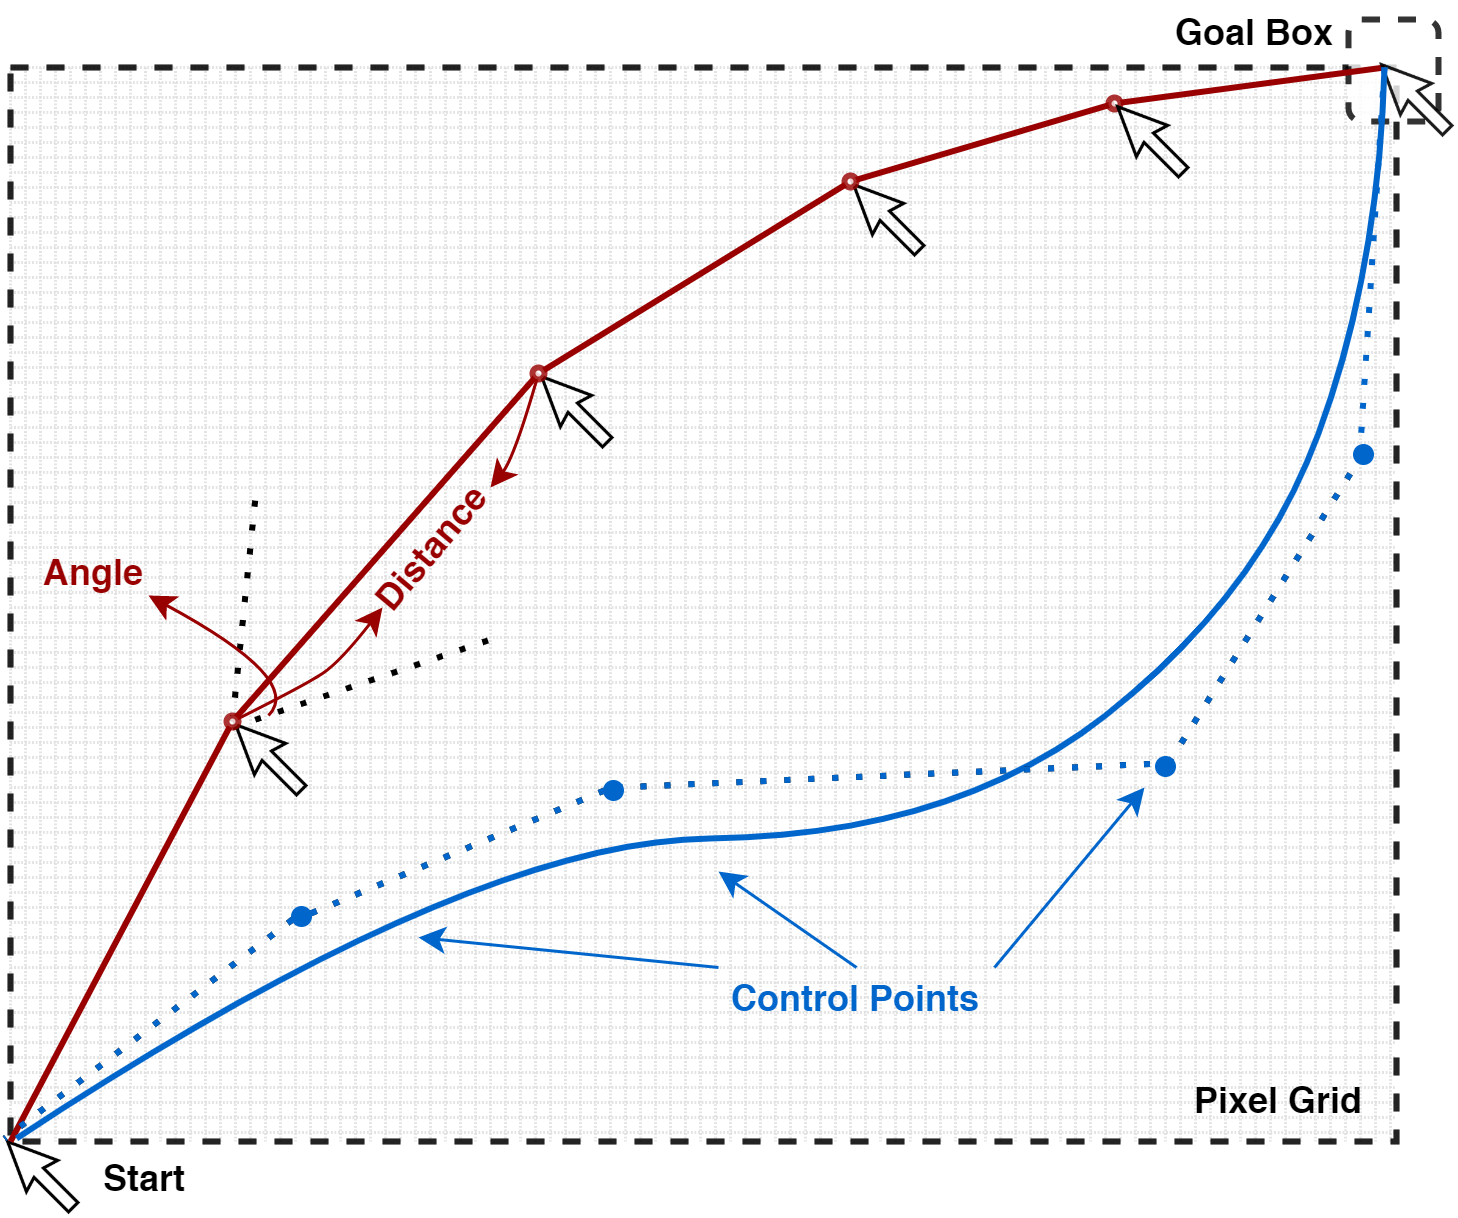
\includegraphics[width=0.95\columnwidth]{mouse.png}}
\caption[Agent controlled mouse movement.]{Agent controlled mouse movement. In red and blue are Piecewise and Bézier trajectories respectively.}
\label{mouse}
\end{figure}

\emph{Bézier.} We define a mouse trajectory from points $A \rightarrow B$ along the Bézier curve, generated by control points randomly selected within the ranges  $[A_x,B_x], [A_y,B_y]$.
Bézier curves are ideal for generating smooth, easily parameterizable trajectories and are commonly used in computer graphics and robotics \cite{tharwat2019intelligent, wang2020using}; a good fit for human-like mouse control.
The agent controls 4 continuous values, which are rescaled to the appropriate range -- listed timings are in seconds:
\begin{itemize}
  \item Duration $d \in [0.5,1.5]$ that defines the trajectory speed.
  \item Hover $h \in [0.2,1.1]$ for the time between the end of the trajectory and the mouse click.
  \item Press $p \in [0.05,0.55]$ for the duration of the mouse button press.
  \item Delay $t \in [2,10]$ for the pause between each request.
\end{itemize}
A sample trajectory is shown in Figure \ref{mouse}.

\emph{Abstract.} Similar to Bézier mode, the agent in Abstract mode controls four actions, with one key difference.
Instead of controlling delay $t$, at each step the agent now selects between three actions; that is scrolling, typing, or mouse control which is carried out exactly like in Bézier mode.
All actions are parameterized by the duration, hover, and press values, as before.
The value ranges for these actions are determined by studies carried out in related literature~\cite{dhakal2018observations, katerina2018mouse}.
For more details on these actions, refer to Appendix \ref{appendix:b}.

\textbf{Reward}. The reward function represents the desired behavior or goal for the agent to achieve.
Since the score in our case is influenced by various factors and can be a noisy signal, a simple reward mechanism is the most practical approach.
In Bézier and Abstract modes, the reward is calculated as the difference between the latest received score and the average cumulative score the agent has received during the current episode:

\begin{equation}
\begin{aligned}
    r_{BA} &= s_t-\overline{(s_{t-1}+\dots+s_0)}\\
\end{aligned}
\label{eqn:reward}
\end{equation}

where $s_t$ is the score at step $t$

In Piecewise mode, the reward is provided at the end of a trajectory/episode and is a weighted average of 3 terms: the difference between the current and last score, the amount of steps taken in order to incentivize precise trajectories, and a small constant term if the score remains high:

\begin{equation}
\begin{aligned}
    r_P &= s_t-s_{t-1} - 0.001\cdot N_t + 0.01\cdot h_t\\
    h_t &=
    \begin{cases}
      1, & \text{if}\ \geq 0.7\\
      0, & \text{otherwise}
    \end{cases}
    %r_1 &= w_1(s_t-s_{t-1})\\
    %r_2 &= -w_2 \cdot N_t\\
    %r_3 &= w_3 \cdot s_t, \forall s_t \geq 0.7\\
\end{aligned}
\label{eqn:rewre}
\end{equation}

where $s_t$ is the score at episode $t$ and $N_t$ is the number of steps in episode $t$.

\subsection{Algorithm}


To select an appropriate \gls{RL} algorithm, we must consider the environment's properties.
Since both the state and action spaces are continuous, traditional value-based methods like Q-learning are computationally impractical.
We thus opt for policy-based approaches that optimize the policy $\pi_\theta(a|s)$ directly, where $\theta$ is usually approximated with neural networks.
These methods have driven recent breakthroughs in dynamic system control, 3D locomotion, and game playing, where the neural network learns the optimal action $a$ for a given state $s$.
From the available policy-based approaches, we conducted our experiments with the \gls{PPO} algorithm, specifically the PPO-Clip variant.
The reader is referred to Chapter \ref{ch:background} for more details on the PPO agent and to Appendix \ref{appendix:a} for its architecture and hyperparameters.

The learning process for the Abstract agent is outlined in Algorithm \ref{alg:abstract}, where: $n$ is the number of actions taken between each score request, $u$ denotes the number of steps between updates to the neural network that parameterizes the policy, $M$ is the total number of episodes, $T$ is the maximum number of steps in an episode, and $a$ is the selected action.
The pseudocode for Piecewise and Bézier agents is included in Appendix \ref{appendix:a}.
To navigate web pages and the system interface, all agents are given $x,y$ values corresponding to absolute screen coordinates.
If the screen location is known in advance, the coordinates are hardcoded; otherwise, they are determined using our browser extension, which retrieves the location of HTML elements.

\begin{algorithm}
\SetAlgoLined
 Set number of steps $n$ per request\;
 Set policy update frequency $u$ in steps\;
 \For{episode $e$ = 1, 2, ... $M$ do}{
   Get initial score $S_0$\;
  \For{step $t$ = 0, 1, ... $T$}{
   Select action $a$\;
   Select duration $d$, hover $h$, press $p$\;
   Perform action $a$ parameterised by $d, h, p$\;
   \If {$t\pmod{u}== 0$}{
    Update policy and value networks based on Eq. \ref{appendix:objective} and Eq. \ref{appendix:value}\;
   }
   \If {$t\mod n == 0$}{
    Get score $S_t$\;
    Set $r_t$ based on Eq. \ref{eqn:reward}\;
   }
  }
 }
 \caption{PPO-Clip Abstract}
 \label{alg:abstract}
\end{algorithm}

\section{Evaluation}
\label{sec:evaluationrere}

In this section, we detail our empirical evaluations and present the results.
For the automated experiments, we use Firefox, Chrome, and Chromium as browsers, along with a VPN service to shuffle our IP between browsing sessions.
To account for the score bias introduced by privacy settings, we define two distinct configurations for browsing sessions: one with third-party cookies disabled and private/incognito browsing enabled -- and one vice versa.
These settings reflect the different levels of privacy-conscious browsing behavior and introduce variance in order to observe their effect on the score.
Within each session, these configurations are kept constant as they represent the static, invariant aspect of browsing; our focus is to analyze how the risk analysis system responds to controlled, interactive behavior.
To maintain methodological validity, browsers retained no state or information between sessions: when private/incognito mode was disabled, cache and cookies were cleared after each session.

\subsection{Manual Assessment}
\label{sub:empirical}

Throughout our experiments, we launch browsers with different configurations on the same machine to investigate potential tracking or cross-browser fingerprinting \cite{boda2011user}.
According to Google and Google Analytics documentation, Google can track unique IDs via NID and SID cookies, for user authentication, fraud prevention, targeted advertising, and other purposes.
For the average web user, a practical yet counterintuitive method to avoid tracking is to reveal more, rather than less, private information, as privacy-conscious settings can make users more conspicuous.
Previous work~\cite{sivakorn2016robot} explored the browser checks reCAPTCHA v2 performs, among them canvas fingerprinting \cite{mowery2012pixel}.
These checks are used to detect web automation frameworks or identify the browser version, with discrepancies flagged by comparing results to the reported user-agent string.
In both our manual assessment and automated evaluation, we found no evidence of tracking or any negative impact on the reCAPTCHA score when the user-agent string was manipulated.

Before conducting the automated evaluation, the first step is to observe how the risk analysis system responds to different browser configurations, the presence of cookies, different IP addresses, and most importantly, user behavior during browsing. 
We categorize the information provided to the system into \emph{static} and \emph{dynamic} components.
By holding all but one feature constant and varying the others, we gain practical insights into how each factor influences the score assigned to each request. Specifically, we observe that:

\begin{itemize}
  \item Google cookies (GRECAPTCHA, NID \& SID) and enabled cookies in general have a decisive role in increasing the system's confidence that the user is indeed human. This is to expected, as cookies track legitimate user activity over time.
  Our experiments with static features show that they affect the overall confidence of the system: when confidence is high, dynamic features have little observable effect; conversely, when the confidence is low they appear to have a strong influence on the score.
  This low-confidence setting is what we aim to induce and exploit to learn evasive human-like browsing behavior.
  \item When starting from a low score, something much more common with cookies disabled, we can reliably increase the score by performing typical browsing activity, such as clicking, scrolling, typing in input fields, and navigating to subpages.
  \item Starting from a high score, the score can be reduced by either overloading the webpage with requests or by performing in bot-like actions using mouse and keyboard automation.
\end{itemize}

The scores returned by reCAPTCHA v3 are coarse-grained, limited to four discrete values: $S \in \{0.1, 0.3, 0.7, 0.9\}$.
A coarse-grained score provides two advantages in a Captcha system: (i) it simplifies the process for web administrators to set thresholds, and (ii) it reduces the amount of information revealed about the model’s decisions—similar to gradient masking in adversarial \gls{ML}.
Although the internal confidence states of the risk analysis system are not directly observable, their effects can be inferred through score behavior: high volatility within a session suggests low confidence, whereas low volatility indicates high confidence.
From our empirical observations, we identify two additional states that may overlap with the high confidence state:

\begin{enumerate}
\item \emph{Score saturation}. Saturation occurs when the risk analysis system has a high level of confidence that the user is human.
This confidence can extend to unrelated requests from other users, making the score unresponsive to dynamic user behavior within the session.
\item \emph{Score depletion}.
Depletion reflects a high confidence that the user is a bot, where all requests in the session receive the minimum score. This can result from excessive requests -- of the variables we control is their frequency -- and may extend to unrelated requests, regardless of their origin.
\end{enumerate}

This score behavior is consistently observed in both manual and automated experiments.
From an adversarial perspective, a low-confidence state is desirable for learning automated solutions, as it makes the score more responsive to user behavior.
It then follows, that high confidence states can serve as a deterrent against automated solutions; this is explicitly acknowledged by Google for reCAPTCHA v2.
In Google's Vulnerability Reward Program\footnote{https://bughunters.google.com/learn/invalid-reports/google-products/4539275112349696}, they advise against submitting reports when reCAPTCHA accepts invalid responses to challenges.
To combat automated solutions, if the system is highly confident a user is human (i.e., in a high-confidence or saturation state), it may accept even incorrect answers.
Conversely, if it is confident a user is a bot, it rejects even correct answers.
The rationale is that consistently accepting correct responses and rejecting incorrect ones simplifies the challenge for adversaries, making it easier to bypass.

\subsection{Automated Evaluation}
\label{sec:auto}

In all our experiments the automation is performed in a fully graphically enabled manner -- no headless browsers are used -- with user browsing behavior simulated by programmatically controlling the mouse and keyboard.
Over a period of 15 months, we submitted more than 70,000 requests.
During this time, we progressively refined our agents to incorporate more general capabilities, enabling them to better emulate abstract, human-like browsing behavior.
To assess transferability effectively, and given the progressively more general agent capabilities, we conduct our evaluation in a cascading manner on three distinct web environments, as introduced in Section \ref{sec:approachre}:

\begin{itemize}
    \item Our self-hosted \textbf{Website A}, which experiences minimal traffic aside from a few researchers, allowing us an unconstrained request budget. Here, the Piecewise agent was both trained and tested, while the Bézier agent was solely in training mode.
    \item External \textbf{Website B}, a site with significant web traffic. On this website, the Bézier agent trained on Website A was tested to evaluate its transferability, while the Abstract agent was in training mode.
    \item External \textbf{Website C}, a high-traffic site with reCAPTCHA v3 already integrated for bot protection. The goal here was to assess how effectively the Abstract agent, trained on Website B, could evade detection.
\end{itemize}

The practical difference between training and testing mode is whether the parameters of the policy network are updated, i.e. whether acutal learning occurs.
Alongside the RL-enabled agents, we implemented and evaluated a \textit{Baseline} agent, which differs in two key ways: mouse movements are performed in a naive manner, either instantaneously or in a straight line between the origin and destination, and no parameter updates or learning take place.

\textbf{Website A}. On this website, we deployed reCAPTCHA v2 alongside v3 to compare their behavior during evaluation.
As shown by \cite{sivakorn2016robot}, when reCAPTCHA v2 is highly confident that a request is submitted by a human, it resolves to ``no Captcha reCAPTCHA'' that lets the user proceed without presenting a challenge.
Interestingly, reCAPTCHA v2 never resolved to "no Captcha" mode when v3 was in a depletion state. Surprisingly, it also often failed to do so even when v3 was in saturation. This suggests that the risk analysis systems behind reCAPTCHA v2 and v3 may differ in how they process collected data and build risk profiles.

The primary goal on this website is to assess the feasibility of automating reCAPTCHA v3 evasion, and determine whether we can learn from the score that the risk analysis system generates.
To test the hypothesis that the scoring system can be exploited, we use a \gls{VPN} service to intentionally initiate sessions that begin from a low score $s < 0.5$; over two thirds of those sessions occur with cookies disabled and private/incognito mode.
Statistically, low-starting sessions demonstrate significantly higher score volatility -- about twice as much, suggesting low-confidence states are more sensitive to user interactions.

In Figure \ref{spps} we illustrate the score evolution averaged over all such sessions, for each methodology we employed.
As sessions can have variable length, we normalize the time axis to a fixed $0-100\%$ range, and we calculate the average over this range.
There is a clear divide in performance between Baseline and both Piecewise and Bézier agents.
For the latter two, the score has a clear upwards tendency that on average surpasses the typical detection threshold within 20-25\% of a session's duration.
We observe a clear drop towards the end in the Bézier progression due to some sessions reaching more than 200 requests where the otherwise consistently high scores suddenly deplete to 0.1.
This is strong evidence that the temporal dynamics of incoming requests are taken into consideration, especially since it occurs at the \emph{same} time irrespective of which session we submit the requests from.
Figure \ref{swos} plots the average cumulative score each methodology achieves over the period of evaluation.
Once again there is a clear divide between the Baseline and the \gls{RL} enabled agents, with Bézier being the approach getting most consistently high scores.

\begin{figure*}[ht!]
  \centerline{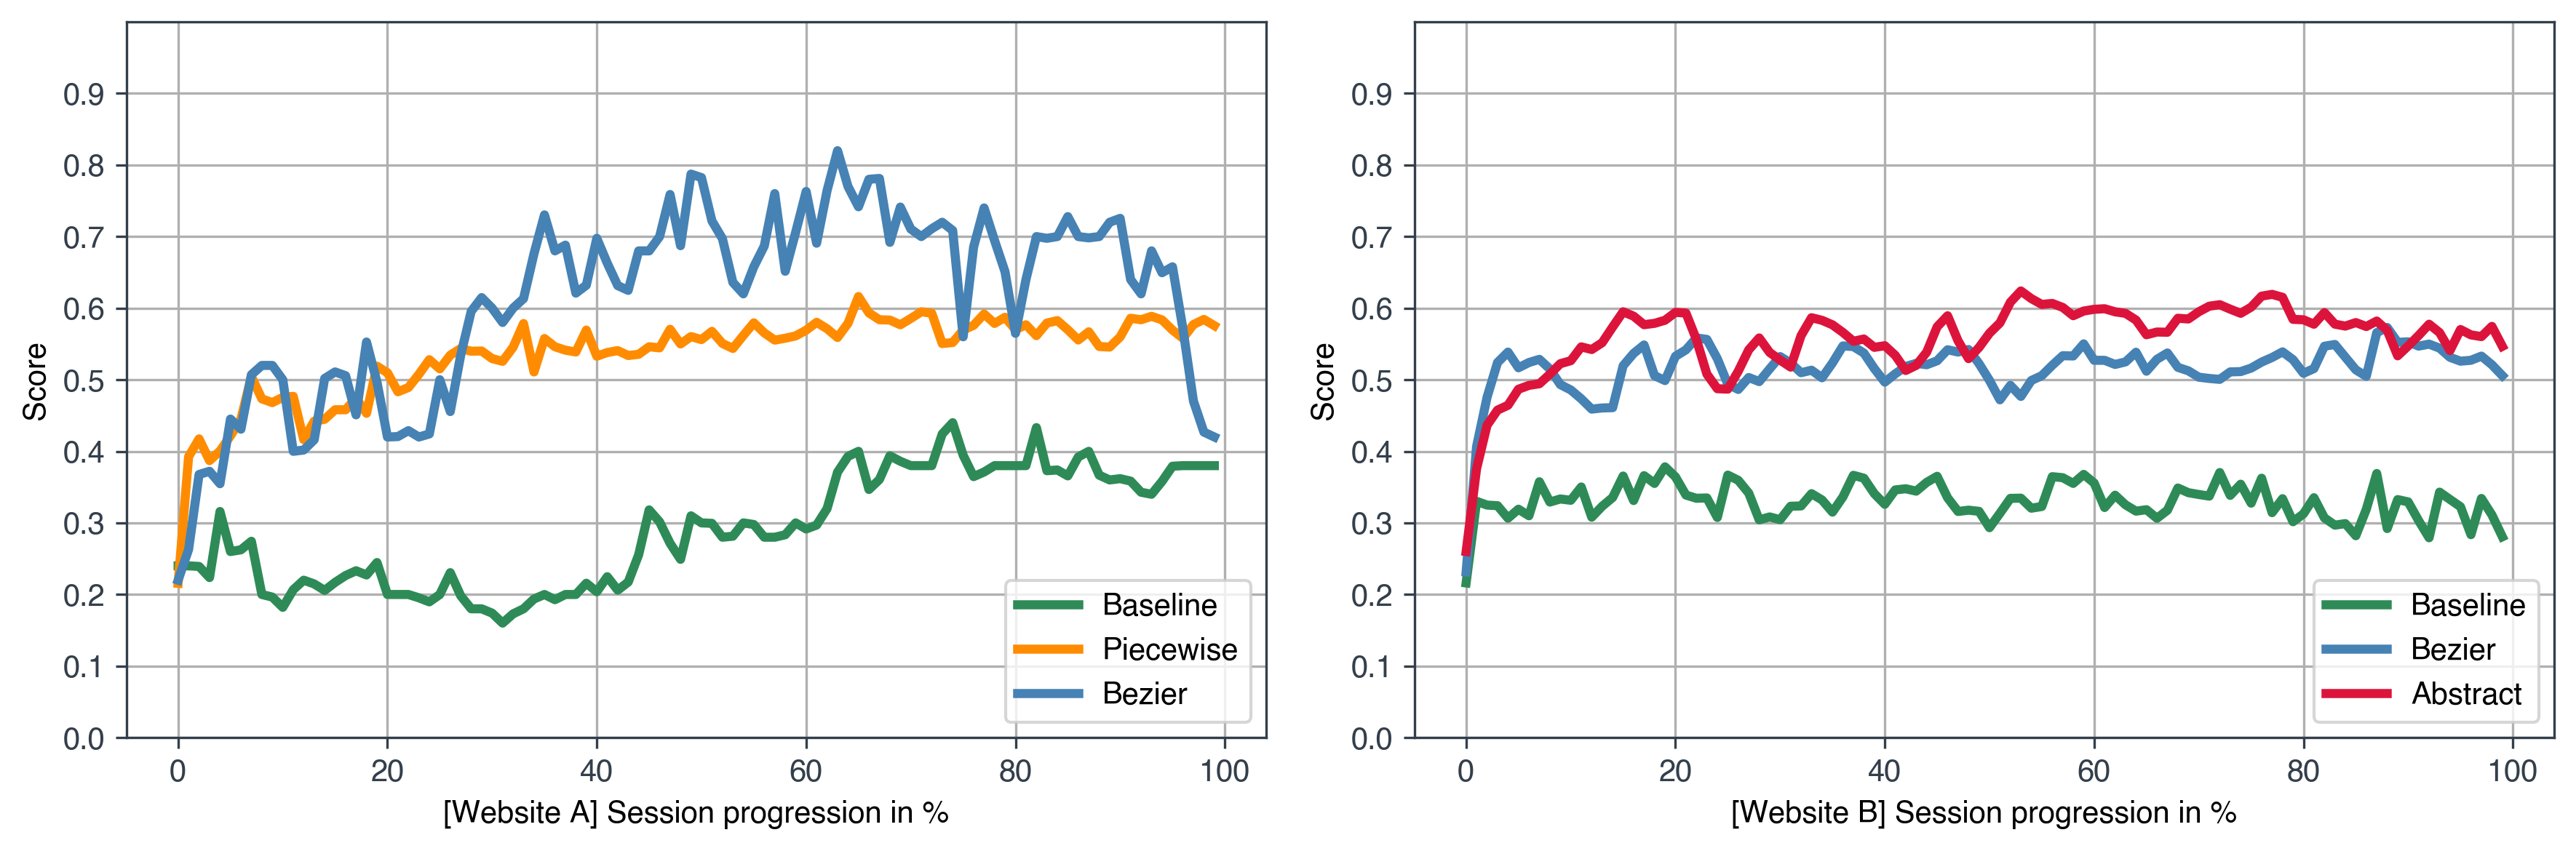
\includegraphics[width=0.95\textwidth]{SPPS.png}}
  \caption[reCaptcha score evolution in sessions initially flagged as bot]{Score evolution in sessions initially flagged as bot, on Website A and Website B.}
  \label{spps}
  \end{figure*}

\begin{figure*}[ht!]
\centerline{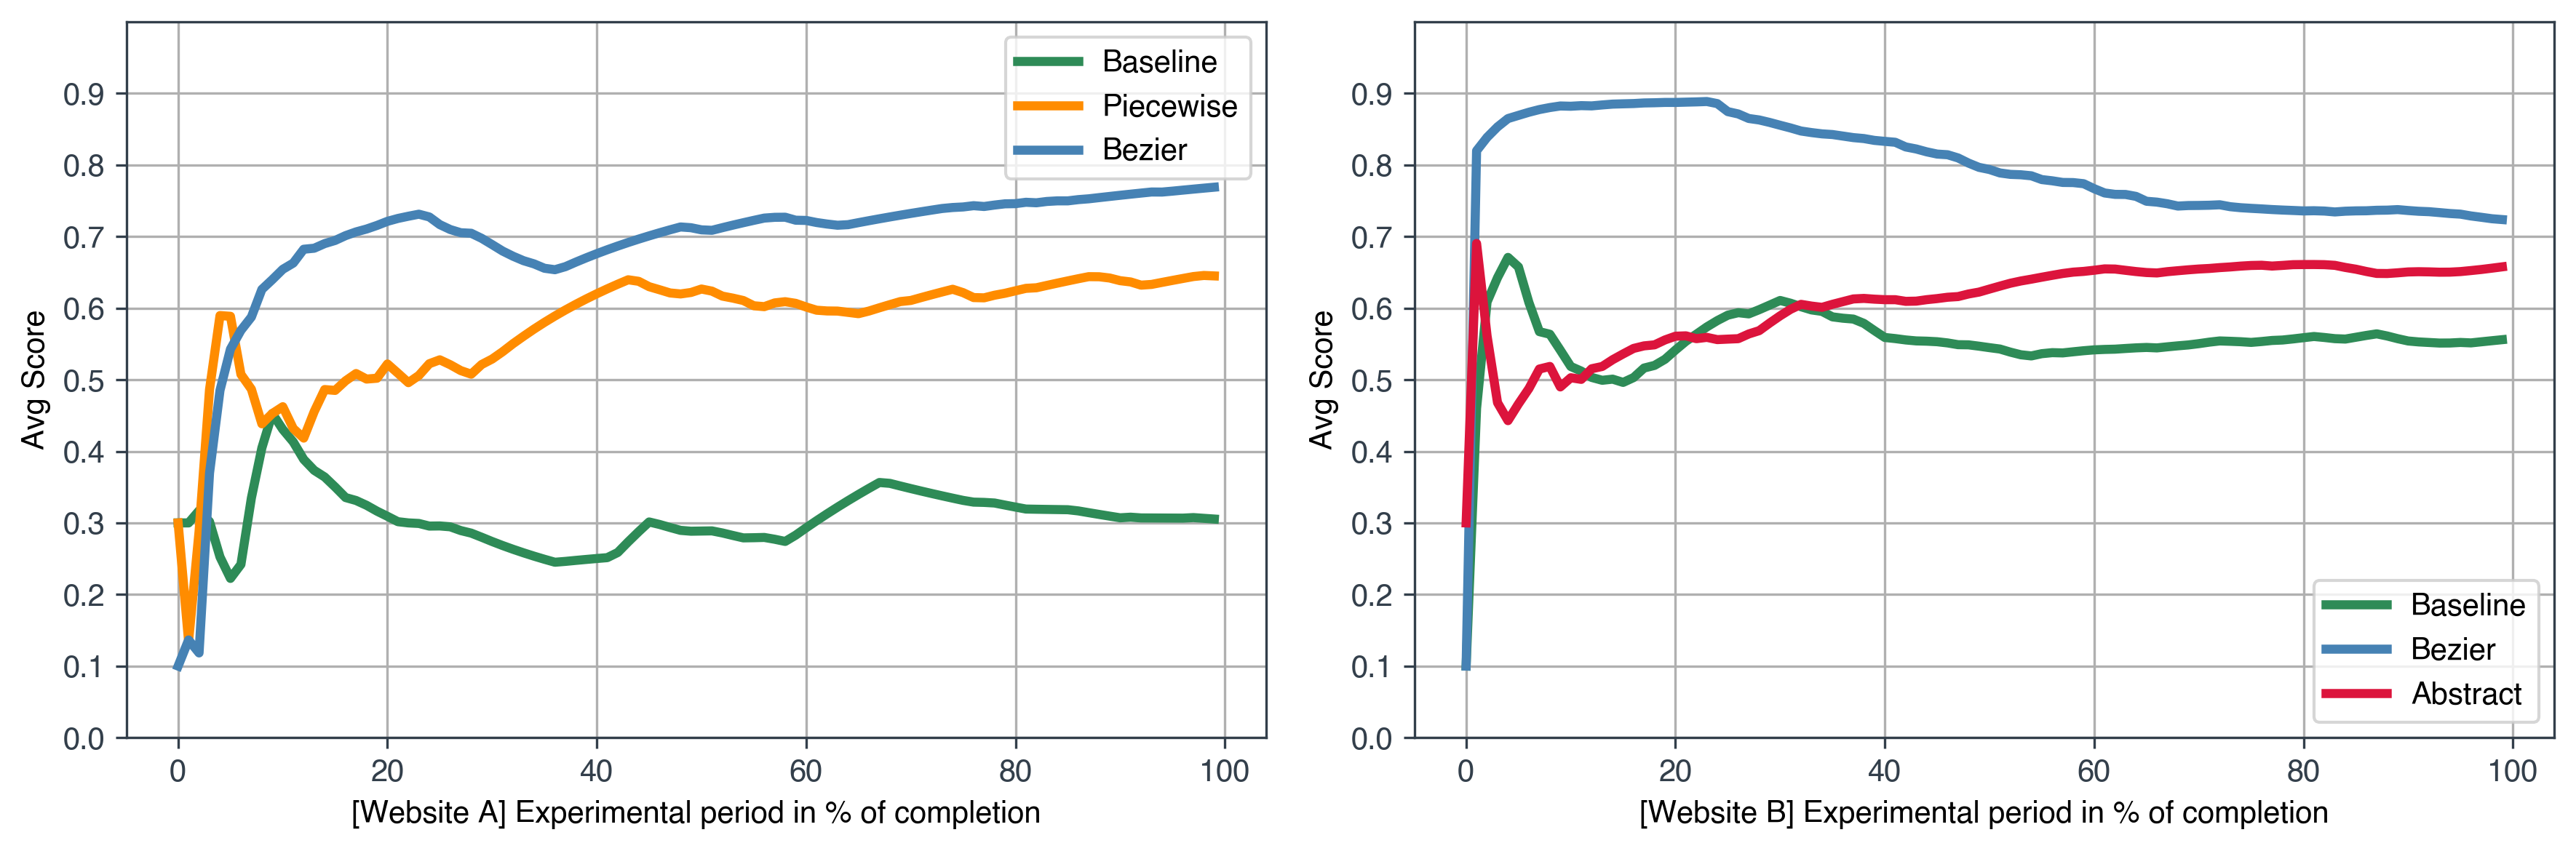
\includegraphics[width=0.95\textwidth]{SWOS.png}}
\caption[Average cumulative score over the period of evaluation.]{Average cumulative score over the period of evaluation, for Website A and Website B.}
\label{swos}
\end{figure*}

\textbf{Website B}. Since website A is practically an artificial web environment, offering ease of access and unlimited querying, it does not fully represent a real-world scenario where the risk analysis system adapts based on actual traffic patterns.
To properly assess the capabilities of our automation, we transition to Website B, which experiences live web traffic.
As detailed in Section \ref{sec:approachre}, in coordination with the administrators we deploy reCAPTCHA v3 on Website B and allowed it to observe traffic for one week to avoid skewing its patterns.
In this setting, we evaluate how well the top-performing agent trained on Website A transfers to this new environment, without using the scores for further retraining or fine-tuning.
Additionally, we ascertain whether an even more general and evasive model can be learned.

In Figure \ref{spps} we illustrate the score evolution averaged over all sessions that start below the bot threshold -- 96 out of 180 -- for each methodology we employed.
We observe a clear but less prominent gap between the Baseline and the \gls{RL} enabled agents.
In this environment saturation and depletion still occur but differently than on Website A.
While it is still possible to deplete the score due to an overabundance of requests, when it happens it concerns only the IP address where the requests were submitted from and does not propagate to others.
The sessions where the score reached depletion due to excessive requests were less than 3\% of the total.

Figure \ref{swos} illustrates the average cumulative score each methodology achieves over the period of evaluation.
One thing we immediately observe is that Bézier performs the best out of the box, however Abstract diminishes the gap over time as the Bézier agent no longer updates its parameters.
Notably, in this web environment the baseline performance is comparable to the \gls{RL} agents.
This indicates that even a rudimentary GUI-enabled automation can be sufficient to consistently evade reCAPTCHA v3 detection.

\textbf{Website C}. After concluding our experiments on Website B, we aim to assess the broader threat posed by our \gls{RL}-enabled automation on the web.
The best candidate for this is the Abstract agent, which incorporates common browsing behaviors that were previously scripted when needed, making it the most general model we developed.
The next step is to evaluate its evasive performance and determine how well it transfers to websites with susbtantial traffic.
Furthermore, our intention is to obviate any form of learning and transition to a fully black-box scenario.
Website C is an ideal candidate as it receives two orders of magnitude more daily traffic than Website B.
Instead, there is only a binary indicator showing whether the score exceeded an unspecified threshold, reflecting real-world attack scenarios where access to scores is unavailable, only the binary verdict if further verification is required.
Whereas on previous websites we tracked the average score, on Website C we report the percentage of requests that go undetected, referred to as the evasion rate.

We evaluate the Baseline and Abstract agents in two key scenarios, representing the worst and best starting points for the adversary: sessions initially flagged as bot (low starting) and those not flagged (high starting).
On Website C, compared to Websites A and B, it is significantly harder to find low-starting sessions.
The results, summarized in Table \ref{tab:requests},
show a marked performance difference between the Baseline and Abstract agents in low-starting sessions, while the gap is smaller in high-starting sessions.
In high-starting sessions, which adversaries can more easily initiate, the Abstract agent achieves an evasion rate of 99.6\%, while even the Baseline agent reaches an evasion rate of 84.3\%.
These results highlight a considerable weakness in reCAPTCHA v3's bot mitigation, and a clear vulnerability that an attacker with sufficient resources can exploit.

\subsection{Explainability}

Despite the overall success of our approach in evading detection and revealing a core vulnerability in the bot detection system, several open questions remain:
\begin{itemize}
    \item What does the risk analysis system behind reCAPTCHA v3 score exactly?
    \item Apart from demonstrating the vulnerability itself, can we obtain a deeper understanding of what is happening within the black box?
    \item Which aspects of online behavior influence the score, and to what extent does each factor contribute?
\end{itemize}

During the evaluation on Website B, we registered about 13K requests in total.
From these requests, we generated a dataset where each instance contains the following information:
\begin{enumerate*}
    \item The duration for which actions execute.
    \item The hover timing.
    \item The press timing.
    \item The delay between successive requests.
    \item The presence of cookies.
    \item The frequency of requests.
    \item The time in the day.
    \item The day of the week.
    \item The number of different actions used.
    \item The total number of requests submitted in current session.
    \item The score that the request got.
\end{enumerate*}

In gain insights into how reCAPTCHA v3 scores requests, an intermediary step is to extract a functionally equivalent model that mimics the decision-making process of reCAPTCHA v3 \cite{jagielski2020high, bastani2017interpreting}.
The extensive data we collected during our experiments provided such an opportunity.
We train Random Forest (\gls{RF}) classifiers and regressors~\cite{liaw2002classification}, using the aforementioned features as independent variables and the score as the target.
In the classification task, we achieved a mean accuracy of $87.5\%$, and in the regression task an $R^2$ of $0.82$. 
An $R^2$ of $0.82$ means that the model cannot explain $18\%$ of the variability in the outcome.
This is anticipated, as Google has access to a broader range of information that we cannot account for, such as IP reputation, deviations from heatmaps generated by Google Analytics, and spatial, temporal, or entropic aspects of user behavior.
These are either missing or confounding variables, and we emphasize that statistical analysis can suggest correlations but does not imply causality~\cite{scholkopf2019causality}.

\begin{figure}[b]
\centerline{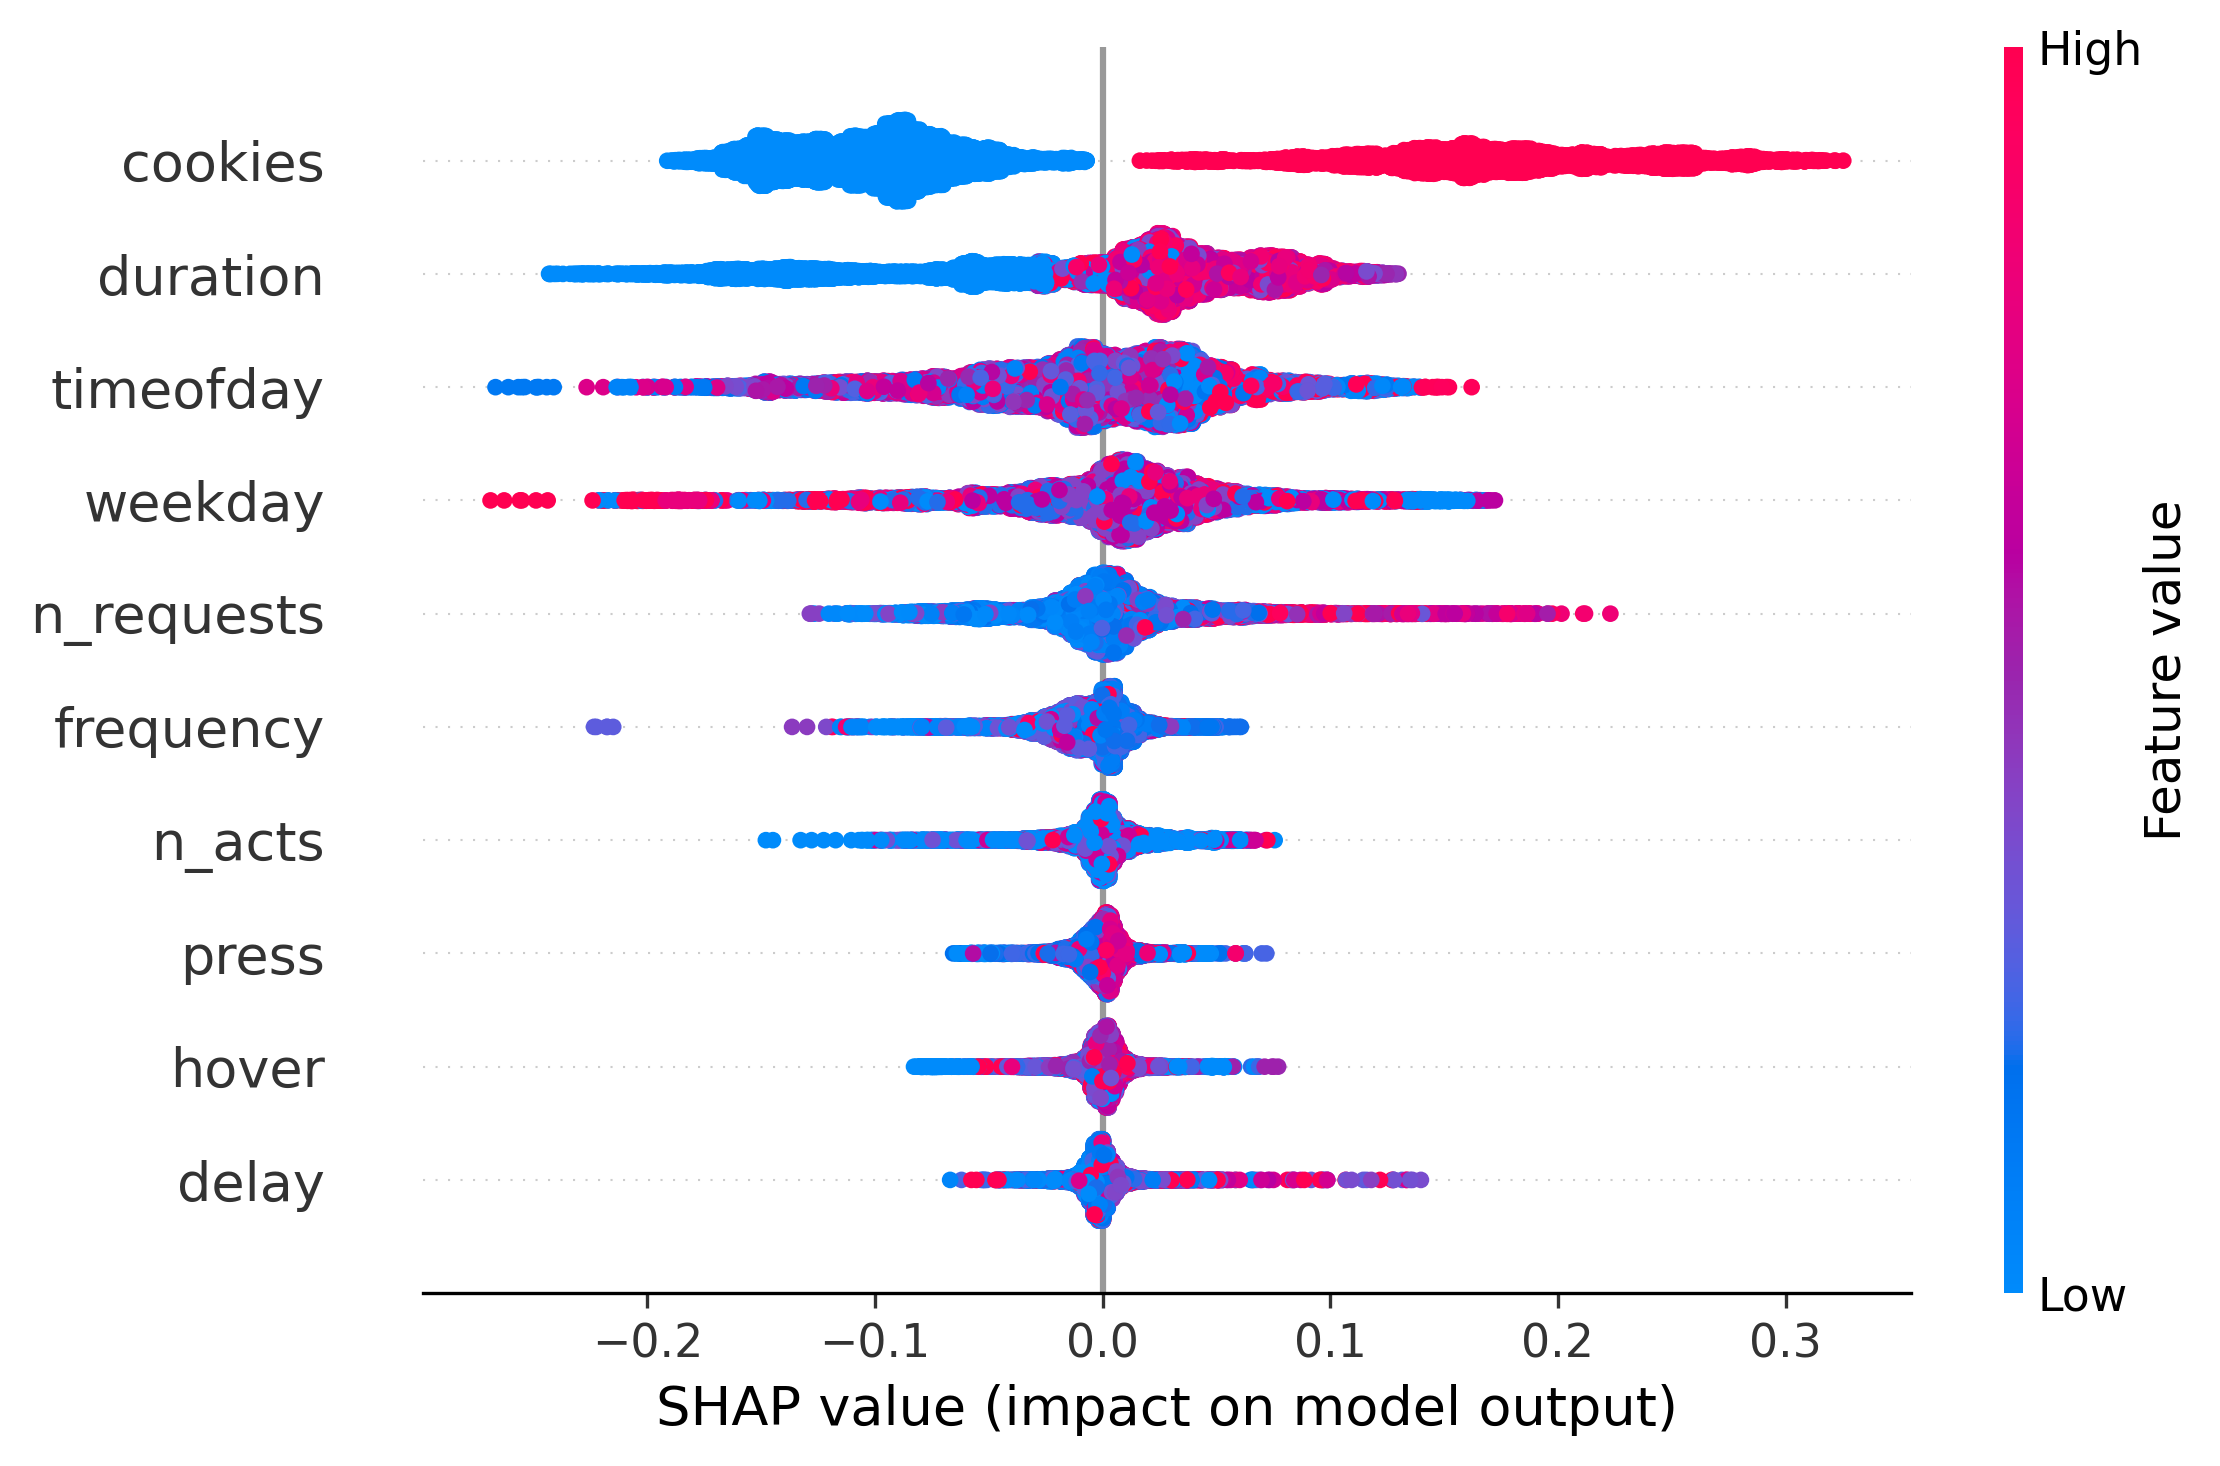
\includegraphics[width=0.95\columnwidth]{SHAP.png}}
\caption{Shapley values for all features, depicted in descending order of importance}
\label{shap}
\end{figure}

Our goal is not to extract a high-fidelity replica of the reCAPTCHA v3 risk analysis system, but rather to gain insights into how various factors influence the score, based on our initial assumptions.
To achieve this, we utilize SHapley Additive exPlanations (SHAP), a robust framework for  \gls{XAI}.
SHAP is a game theoretic approach that explains the output of any \gls{ML} model.
SHAP connects optimal credit allocation with local explanations using the Shapley values, i.e. the average of the marginal contributions of the features, across all the feature permutations~\cite{lundberg2017unified}.
We note here that by following an experimental protocol, bias is inadvertently introduced into the collected data.
For example, the impact of cookies is likely exaggerated, as we specifically searched for low-starting sessions, which occur more frequently when cookies are disabled.

Figure \ref{shap} demonstrates how each variable influences the score, in descending order from most to least influential.
The presence of cookies is the most influential, indicating that the risk analysis system has a clear bias between more and less privacy-aware web browsing behavior.
What is interesting though is duration at the second spot and that it is positively correlated with the score.
This indicates that short or instant actions are biasing the score to lower values.
Time of day and weekday are also influential; their influence is most probably overestimated as we unintentionally introduce some bias by following typical (mostly) office activity.
The number of requests can appear counter-intuitive at first; while a few high values are correlated with low scores, indicating depletion, the feature is mostly positively correlated with score, indicating that longer and human-like activity is a strong predictor of higher scores.
The number of actions shows a slight and positively correlated influence, corroborating our findings that put the Abstract mode a step above Bézier.
What is surprising however is that mouse button press, mouse hover, and the delay between requests have little to no impact to the model.
The value ranges for press and hover were defined to match typical human ranges, thus the score might be completely unswayed by them, as far as the model is concerned.

\textbf{Computational cost}. Throughout our experiments, the most computationally demanding agent was Piecewise, as it controls actions at a rate of 50 FPS required for seamless trajectories.
The computational bottleneck here is the neural network behind the agent policy, and the average inference time on an Intel i7-7700 CPU was $5 \times 10^{-4}$ seconds which could theoretically support up to 2000 FPS control.
Regarding the implementation and evaluation platforms, all scripts and \gls{RL} agents were coded in Python while a browser extension written in JavaScript was used to retrieve scores -- all experiments were carried out on a dedicated desktop machine with Ubuntu 18.04.

In Table \ref{tab:requests} we report the summary on the scores, numbers of requests, and overall traffic, across all experiments and for each of the websites.
Over a period of 15 months, our \gls{RL} enabled methodology successfully used the risk analysis system behind reCAPTCHA v3 to learn evasive models of web browsing, while submitting high numbers of requests commensurate to the total traffic a website attracts.

\begin{table*}
\centering
   \begin{tabular}{lccc|ccc|cc}
    \toprule
    &
      \multicolumn{3}{c}{Website A} &
      \multicolumn{3}{c}{Website B} &
      \multicolumn{2}{c}{Website C}\\
      & \small {Base} & \small {Piece} & \small {Bézier} & \small {Base} & \small {Bézier} & \small {Abstract} & \small {Base} & \small {Abstract}\\
      \toprule
    $S_L$ & 0.22 & 0.52 & 0.60 & 0.33 & 0.60 & 0.58 & 20.8\% & 70.1\%\\
    $S_T$ & 0.31 & 0.65 & 0.77 & 0.56 & 0.72 & 0.66 & 51.6\% & 90.0\% \\
    $S_H$ & 0.52 & 0.71 & 0.83 & 0.73 & 0.86 & 0.80 & 84.3\% & 99.6\% \\
    \midrule
    $R_T$ & 2.6K & 21K & 8K & 6.3K & 4.4K & 2K & 8.6K & 12.4K\\
    $R_D$ & 130 & 231 & 244 & 203 & 182 & 89 & 866 & 773 \\
    $R_S$ & 101 & 140 & 144 & 93 & 75 & 37 & 208 & 122\\
    $D_S$ & 203 & 761 & 526 & 40 & 71 & 37 & 68 & 136\\
    % $N_D$ & & 92 & 33 & 31 & 24 & 22 & & & & 8\\
    \midrule
    $T_T$ & -- & -- & -- & 12.3K & 9.4K & 9.3K & 328K & 413K \\
    $T_D$ & -- & -- & -- & 398 & 390 & 421 & 33K & 26K\\
    \bottomrule
  \end{tabular}
  \caption[reCaptcha requests and scores per website and agent.]{Requests per website and agent. $S_L$, $S_T$, $S_H$ are the average score for low starting, total, and high starting sessions respectively. For Website C, $S_L$, $S_T$, $S_H$ denote the evasion rate instead. $R_T$ is the total amount of requests, $R_D$ are the average requests per day, $R_S$ are the average requests per session, $D_S$ is the average session duration in minutes, $T_T$ and $T_D$ are the total and daily amount of traffic during the experiments.}
  \label{tab:requests}
\end{table*}

\section{Discussion}
\label{sec:discussionre}

In this section, we critically reflect on the results and provide further insights into the topic.
Captcha solutions are an essential tool to combat bot proliferation on the internet and the financial or other harm they may cause.
From fraudulent transactions to credential stuffing attacks and click fraud, adversaries stand to gain significantly from developing general, human-like browsing behaviors that can bypass Captcha detection.
The ability to learn such evasive behavior by using a widely adopted Captcha service as an oracle highlights a significant vulnerability that needs to be addressed, as it could form a core component of systems designed to automate web attacks.
Transitioning from one-shot Captcha challenges to continuous behavior monitoring has another implication.
If human behavior and its imitation are indistinguishable to such a detection system, not only is the system inadequate, but it also facilitates the refinement of bot behavior to further perfect this imitation.

In January 2020 Google launched reCAPTCHA Enterprise, where this vulnerability could potentially be more severe.
According to the documentation, reCAPTCHA Enterprise appears to be based on reCAPTCHA v3, with some modifications that intend it towards enterprises.
Like v3, reCAPTCHA Enterprise will never interrupt users with a challenge, but it includes a pricing for every 1K requests submitted above 1M per month.
Additionally, potential customers have to supply personal and company information for a vetting process.
A key difference to reCAPTCHA v3 is that now the scores returned include reason codes.
These codes provide information on the reason reCAPTCHA Enterprise interpreted the interaction that way, in practice embedding explainability into the inference process.
Such reason codes are:
\begin{itemize}
  \item \textit{automation}, when an automated agent is detected.
  \item \textit{unexpected\_environment}, when an illegitimate environment is detected.
  \item \textit{too\_much\_traffic}, when the traffic volume from a specific source exceeds typical values.
  \item \textit{unexpected\_usage\_patterns}, when interactions in the website diverge significantly from expected patterns.
  \item \textit{low\_confidence\_score}, when there is insufficient traffic observed to generate a representative risk score.
\end{itemize}
There are several surprising correspondences between these reason codes and our findings from investigating the reCAPTCHA v3 risk analysis system, such as the code \textit{too\_much\_traffic}.
An adversary with access to such explanations behind the black-box decision would gain a more detailed understanding of how their actions impact the system, providing another learning signal to further optimize policies on.
However, implementing a premium on requests and subjecting customers to a vetting process could act as a deterrent.
This indicates a promising path for future work.

\textbf{Ethics}.
Before deploying reCAPTCHA v3 on Websites B and C, we acquired explicit consent from the owners and administrators.
Regarding the potential impact on these websites, an open question was how will our automated activity affect the scores of unrelated requests and overall user experience, even considering that a low score will not mean escalation to further verification in neither website.
After all, depletion is a prominent phenomenon on Website A, so we wanted to be extra careful when we proceeded to actual websites with considerable live traffic.
In contact with the website administrators, we set an initial conservative threshold on the amount of queries submitted to be in par with the daily traffic, and gradually increased it.
In case of depletion we agreed to slow our requests down to a halt in order to investigate the cause and analyze the impact; something that ultimately did not occur.

\textbf{Responsible Disclosure}.
Regarding the broader impact that our evasion attack could have on Google reCAPTCHA v3, we followed the standard responsible disclosure policy: we notified Google of our findings and the vulnerabilities we discovered in reCAPTCHA v3.
Google responded to our detailed report and acknowledged the vulnerability.
After further investigation on their side, Google has closed the issue without providing a fix and the status code ``intended\_behavior''.
We surmise that acquiring access to backend scores and that fully graphically enabled automation attacks are considered reasonable limitations on the adversary, however at the time of publication these issues were still present.

\textbf{Defenses}. Since our methodology does manipulate HTTP requests or cookies, defenses would fall primarily within the adversarial training paradigm~\cite{tramer2017ensemble}.
This involves training the risk analysis system with data that were specifically created to fool it, with the goal to make it more robust towards adversarial activity.
As the domain of Captchas is considerably different from image classification, adversarial training is not directly applicable.
Irrespective to abstraction or representation, human behavior online is highly diverse making it easier for adversarial examples -- adversarial behavior here -- to blend into the crowd.
As adversarial examples are fundamentally \gls{OOD} data~\cite{geirhos2020shortcut}, proactively modeling them in this context is particularly challenging.
There is however precedent for using adversarial examples as Captchas, as they are resilient to automated solving~\cite{osadchy2017no}.
Ultimately, as long as adversaries can obtain oracle access to the risk analysis system, defenses are limited to obfuscation and rate limiting.
With this access, attackers can iteratively refine their methods, using the oracle as either a discriminator in a \gls{GAN} approach or a reward function to a \gls{RL} algorithm.

\textbf{Limitations}. The most capable agent demonstrates that it is possible to evade detection on a website of which it had no prior knowledge or interaction with.
However, to fully exploit the information leakage in reCAPTCHA v3, and in case the initial evasive policy is insufficient, an adversary would need extended access to the oracle, as evidenced by the score evolution shown in Figure \ref{swos}.
Moreover, while the score returned by v3 serves as a signal that facilitates learning, it is still noisy, and, as Google indicated for v2, may even be intentionally misleading.
If other significant influencing factors are not properly controlled, this noise inherently limits the extent to which effective learning can occur.

In many configurations, such as with low privacy settings, the baseline approach was sufficient to evade detection, unless depletion occurred.
Beyond demonstrating the effectiveness and transferability of our approach, these results highlight the need to deepen our scientific understanding of the strengths and limitations of frictionless Captcha, especially in the presence of adaptive attackers capable of learning from interaction with the detection system.

\textbf{Controversies}. While Captchas are a crucial tool in combating bots and malicious users, they are not without controversy.
Google reCAPTCHA, in particular, has been criticized for being a source of unpaid work to assist in transcribing text and image labeling tasks.
As a competing solution, hCaptcha\footnote{https://www.hcaptcha.com/} was developed with a different approach, sharing the revenue generated from Captcha solving with the website owner.
A more concerning issue arises with frictionless Captchas, such as reCAPTCHA v3 and Enterprise, which collect vast amounts of data by monitoring user interactions on websites.
As automated solving becomes increasingly efficient, Captchas are shifting toward behaviometrics, moving away from tasks like transcribing text or labeling images.
In this case, user behavior itself becomes the focus, no longer to commercialize insights but to be used in Turing tests.

\textbf{Future Work}.
We opt for \gls{RL} as a learning paradigm as it enables optimal behavior without access to gradients; the agent can learn in an immediate, online manner by interacting with the environment.
Our approach and general framework are modular by design to accommodate the learning of any parameters that might affect the risk analysis scoring system, in the case it adapts to observing a broader or different set of information.
As a result, there are two primary promising paths for future exploration:
First, training more capable agents by exploiting the reason codes of reCAPTCHA Enterprise.
Secondly, exploring defenses beyond rate limiting and security by obscurity, in the domains of adversarial \gls{ML} and competitive multiagent \gls{RL}.

\section{Conclusion}
\label{sec:conclusion}
This work presents the first comprehensive investigation of Google reCAPTCHA v3.
Over a 15-month period, spanning multiple websites, web configurations, and attack methodologies, we conduct a black-box analysis and thorough evaluation of the risk scores generated by reCAPTCHA v3.
Our findings reveal that it provides insufficient protection against web automation as we consistently bypassed it with an evasion rate up to 99.6\%.
We evaluate how different aspects of browsing a website protected by reCAPTCHA v3 affect the score.
Static aspects like privacy settings and IP address have a consistent positive or negative impact on the score and remain unchanged during a session.
In contrast, the score is influenced by dynamic, volatile factors tied to user behavior.
Since reCAPTCHA v3 continuously monitors user interactions to differentiate between humans and bots, we exploit this process to develop a general model of automated web browsing that consistently evades detection.

Our study suggests that while the shift towards Captcha services based on continuous behaviometric evaluation is inevitable -- as text and image Captchas are now easier for AI to solve than for humans -— it also introduces vulnerabilities that adversaries could exploit.
The effectiveness of our approach demonstrates the need for more robust bot and automation detection in frictionless, challenge-free Captchas.
As this type of Captcha becomes more widespread, the competition to distinguish between genuine human interaction and its imitation intensifies, underscoring the need for further research into both proactive and reactive strategies to counter such adversarial activity.